\section{Convergence}
There are several factors that contribute to the successful convergence of the polynomial chaos expansion sum with coefficients calculated by quadrature.  The coefficients are calculated as
\begin{equation}
u_p \approx \sum_{\ell=0}^{L} w_\ell U(Y_\ell) \psi_p(Y_\ell).
\end{equation}
Two significant sources of error appear in this calculation: first, the quadrature truncation error from using only $L$ terms in the quadrature set; second, the inherent error in the solver $U(Y)$, which we denote spatial discretization error.  While this assumes the error in the solver is chiefly from the division of the domain into a mesh of finite refinement (for example, using finite element or finite volume methods), it could similarly apply to other solution method errors.
We consider the impact of both quadrature truncation error and spatial discretization error on the convergence of the expansion coefficients.

\subsection{Quadrature}\label{sec:quadconv}
One concern with using stochastic collocation to build the polynomial chaos moments is the appropriate order of quadrature to use.  With Gaussian quadrature, a sum with $n$ terms can exactly integrate a polynomial of order $2n-1$.  The chaos moment expression we integrate is
\begin{align}
u_p &= \int_\Omega U(Y)\rho(Y)\psi_p(Y)dY,\\
  &\approx \sum_{\ell=0}^L w_\ell U(Y_\ell)\psi_p(Y_\ell),
\end{align}
where $\rho$ is the probability distribution of $Y$ and $\psi_p$ is the $p-th$ order basis polynomial.  In the simplest case when $U(Y)$ is a scalar quantity, the order of the expression under the integral is determined solely by the basis polynomial.  Thus a quadrature order of $(i+1)/2$ is the minimum quadrature order necessary to integrate the chaos moments.  In the case $U(Y)$ is highly nonlinear and ill-approximated by even high-order polynomials, the necessary quadrature order required to accurately determine moments is much higher.

As an example of chaos moment convergence as a function of quadrature order, we show the PCESC moments of the 1D diffusion solver critical case for 7th-order quadrature in Table \ref{tab:quadconverge}, as determined by increasing orders of quadrature from the minimum to 12-th order, which assumes $U(Y)$ alone is well-approximated by a 7th-order polynomial.  As can be seen, the lower moments require smaller quadrature orders, and at least order 8 quadrature is necessary to see reasonable convergence for higher moments.  While the mean converges with low-order quadrature, the highest expansion order doesn't converge to discretization error until 10-th order quadrature is used.

Table \ref{tab:1dcrit coeffs} shows expansion moments calculated using quadrature order equal to expansion order for orders up through 31.


\begin{landscape}
\begin{table}[H]
\begin{center}
\begin{tabular}{c | *{8}{l}}
Quadrature Order & $u_0$ & $u_1$ & $u_2$ & $u_3$ & $u_4$ & $u_5$ & $u_6$ & $u_7$ \\ \hline
5 & 1.34648094 & -0.13502447 & 0.02226791 & -0.0045477 & 0.00000000 & 0.00101863 & -0.00092988 & 0.00313821\\
6 & 1.34648100 & -0.13502501 & 0.02227125 & -0.00456451 & 0.0010908 & -0.00027317 &  0.00000000 & 0.00025291\\ 
8 & 1.34648101 & -0.13502506 & 0.02227158 & -0.00456614 & 0.0010978 & -0.00029964 & 9.01120742e-05 & -2.67010906e-05\\ 
10& 1.34648101 & -0.13502506 & 0.02227158 & -0.00456616 & 0.0010979 & -0.00030000 & 9.13419949e-05 & -3.05173759e-05\\ 
12& 1.34648101 & -0.13502506 & 0.02227158 & -0.00456616 & 0.0010979 & -0.00030001 & 9.13732306e-05 & -3.06142832e-05
\end{tabular}
\end{center}
\caption{Chaos Moment Convergence with Increasing Quadrature Order}
\label{tab:quadconverge}
\end{table}
\end{landscape}

\begin{table}[H]
\begin{center}
\begin{tabular}{c | l l l l l}
Moment & SC1 & SC3 & SC7 & SC15 & SC31\\ \hline
0 & 1.34608094 & 1.3464801 & 1.34648101 & 1.34648101 &  1.34648101\\
1 & -0.13145279 & -0.1350169 & -0.13502506 & -0.13502506 &  -0.13502506\\ 
2 & 0 & 0.02222067 & 0.02227158 & 0.02227158 &  0.02227158\\ 
3 & 0 & -0.00431037 & -0.00456614 & -0.00456616 & -0.00456616 \\ 
4 & 0 & 0 & 0.0010978 & 0.0010979 & 0.0010979 \\ 
5 & 0 & 0 & -0.00029964 & -0.00030001 & -0.00030001 \\ 
6 & 0 & 0 & 9.01120742e-05 & 9.13747084e-05 & 9.13746830e-05 \\ 
7 & 0 & 0 & -2.67010906e-05 & -3.06188612e-05 & -3.06187650e-05 \\ 
8 & 0 & 0 & 0 & 1.11868181e-05 & 1.11865704e-05 \\ 
9 & 0 & 0 & 0 & -4.42800671e-06 & -4.42735312e-06 \\ 
10 & 0 & 0 & 0 & 1.89021407e-06 & 1.88853134e-06 \\ 
11 & 0 & 0 & 0 & -8.66874281e-07 & -8.62852707e-07 \\ 
12 & 0 & 0 & 0 & 4.24658199e-07 & 4.15693998e-07 \\ 
13 & 0 & 0 & 0 & -2.18790217e-07 & -1.99976426e-07 \\ 
14 & 0 & 0 & 0 & 1.12938059e-07 & 7.56801496e-08 \\ 
15 & 0 & 0 & 0 & -4.90000878e-08 & 2.05894301e-08 \\ 
16 & 0 & 0 & 0 & 0 & -1.22580841e-07 \\ 
17 & 0 & 0 & 0 & 0 & 2.51097599e-07 \\ 
18 & 0 & 0 & 0 & 0 & -4.18278488e-07 \\ 
19 & 0 & 0 & 0 & 0 & 6.25910592e-07 \\ 
20 & 0 & 0 & 0 & 0 & -8.61060458e-07 \\ 
21 & 0 & 0 & 0 & 0 & 1.09209939e-06 \\ 
22 & 0 & 0 & 0 & 0 & -1.26866179e-06 \\ 
23 & 0 & 0 & 0 & 0 & 1.32892404e-06 \\ 
24 & 0 & 0 & 0 & 0 & -1.21597330e-06 \\ 
25 & 0 & 0 & 0 & 0 & 9.01437926e-07 \\ 
26 & 0 & 0 & 0 & 0 & -4.09433059e-07 \\ 
27 & 0 & 0 & 0 & 0 & -1.70599526e-07 \\ 
28 & 0 & 0 & 0 & 0 & 6.94034499e-07 \\ 
29 & 0 & 0 & 0 & 0 & -9.99892578e-07 \\ 
30 & 0 & 0 & 0 & 0 & 9.71463606e-07 \\ 
31 & 0 & 0 & 0 & 0 & -5.97051529e-07 \\ 
\end{tabular}
\end{center}
\caption{Chaos Moments for 1D Critical Case}
\label{tab:1dcrit coeffs}
\end{table}


\newpage
\subsection{Spatial Discritization}\label{sec:spaceconv}
To see the effect of spatial discretization on coefficient convergence, we consider the quarter core benchmark solver.  We consider five univariate cases.  In each, we vary a different parameter chosen from $\xs{2,c}{1},\xs{2,f}{1},\xs{2,c}{4},\xs{2,f}{4},D_{2}^{(5)}$.  For each parameter, we use the coarsest mesh (11x11) possible in the quarter-core benchmark and plot the expansion coefficients up to order 256, shown in Fig. \ref{fig:2g2d5v coarse cof}.  While the Material 4 and Material 5 properties converge quickly to acceptable levels, the Material 1 properties fail to converge past a magnitude of $10^{-4}$.
\begin{figure}[H]
\centering
   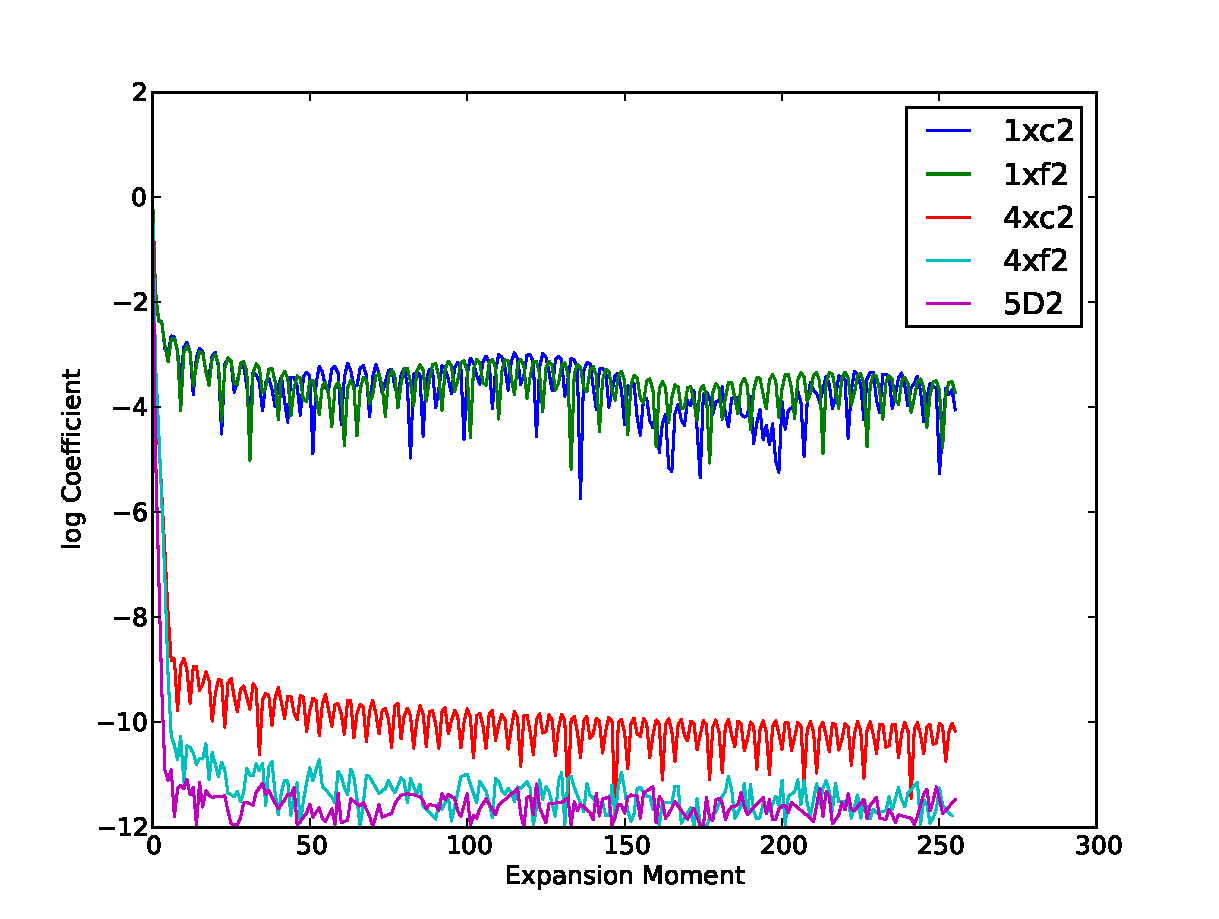
\includegraphics[width=0.7\textwidth]{../graphics/coefficient_decay}
   \caption{Quarter Core Solver Coarse Mesh Coefficient Decay}
   \label{fig:2g2d5v coarse cof}
\end{figure}
To demonstrate the effect of increasing mesh refinement, we consider only the low-energy capture cross section for the first region (1xc2, $\xs{2,c}{1}$).  In each successive refinement $n=(1,2,3,4,5)$ we subdivide each of the 121 regions of the problem into $n^2$ cells, so that for $n=2$ the global mesh is 22x22, and so on.  The results are shown in Fig. \ref{fig:2g2d 1xc2 cof decay}.  With only one additional refinement level, the coefficients converge to acceptable levels.
\begin{figure}[H]
\centering
   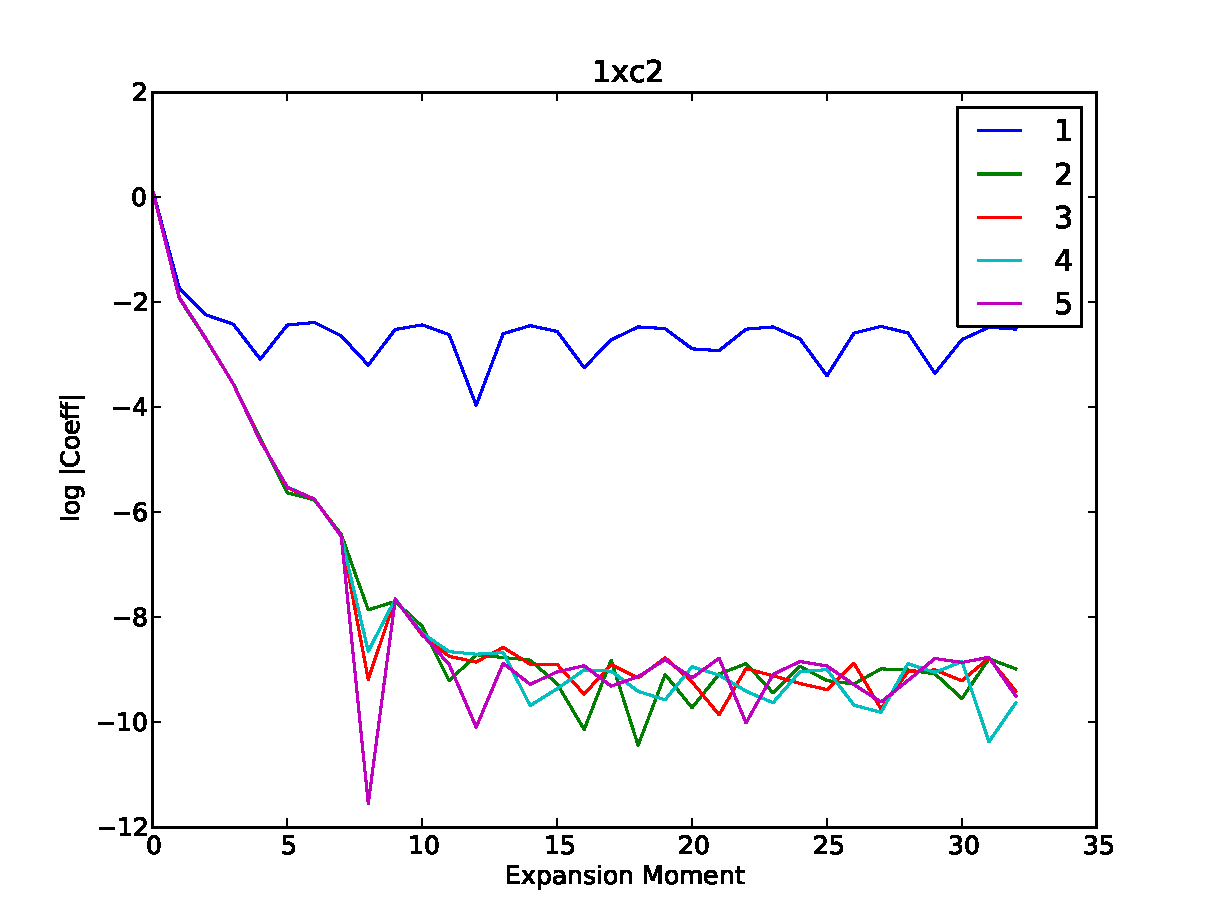
\includegraphics[width=0.7\textwidth]{../graphics/cof_decay_1xc2_meshes}
   \caption{2G2D: Coefficients over Mesh Refinement}
   \label{fig:2g2d 1xc2 cof decay}
\end{figure}
We repeat the original exercise, this time making use of the $n=2$ refined mesh, and see all coefficients converging to an acceptable level after several terms.  The results are in Fig. \ref{fig:2g2d5v fine cof}.
\begin{figure}[H]
\centering
   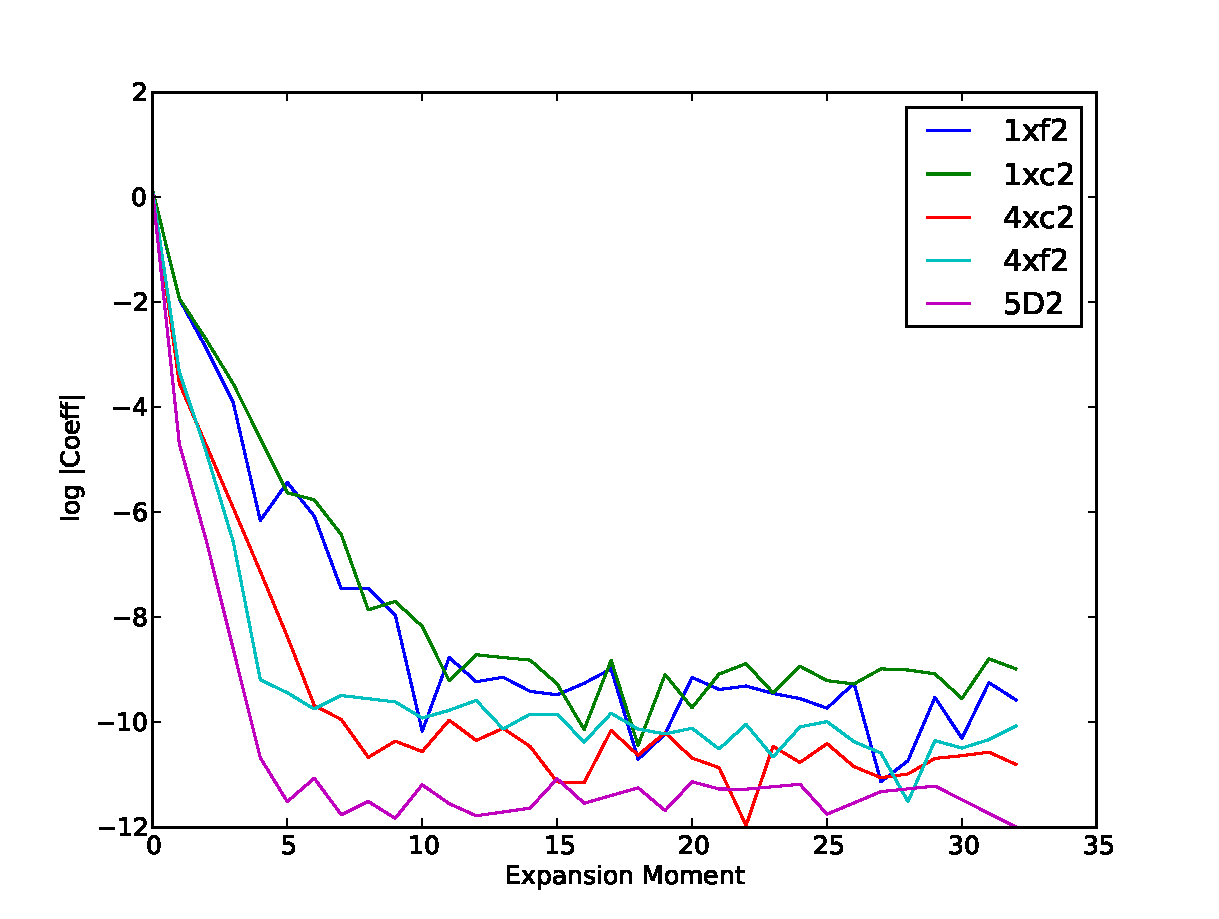
\includegraphics[width=0.7\textwidth]{../graphics/coefficient_decay2}
   \caption{2G2D: Coarse Mesh Coefficient Decay}
   \label{fig:2g2d5v fine cof}
\end{figure}